\documentclass[10pt,aspectratio=169]{beamer}

\usetheme[progressbar=frametitle]{metropolis}

\newcommand{\R}{\mathbb{R}}
\renewcommand{\P}{\mathbb{P}}
\newcommand{\set}[1]{\{#1\}}

\usepackage{tikz}
\usetikzlibrary{shapes}
\usetikzlibrary{plotmarks}
\usetikzlibrary{fit}
\usetikzlibrary{overlay-beamer-styles}
\usetikzlibrary{positioning}
\usetikzlibrary{calc}
\usetikzlibrary{decorations.pathreplacing}
\usetikzlibrary{decorations.pathmorphing}
\definecolor{lightblue}{RGB}{189,216,238}

\usepackage{etoolbox}

\title{Non-Parametric Machine Learning Models for Solar Energy Forecasting}
% \subtitle{}
\date{16.07.2021}
\author{Pavel Zwerschke}
\institute{Karlsruhe Institute of Technology}
% \titlegraphic{\hfill\includegraphics[height=1.5cm]{logo.pdf}}

\begin{document}

\maketitle

\begin{frame}{Table of contents}
    \setbeamertemplate{section in toc}[sections numbered]
    \tableofcontents%[hideallsubsections]
\end{frame}

\section{Model descriptions}

\begin{frame}{NNQF}
    \begin{center}
        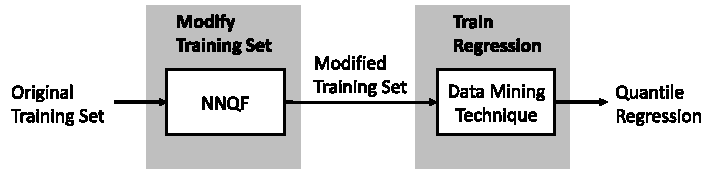
\includegraphics{plots/nnqf_approach.pdf}
    \end{center}
    \begin{itemize}
        \item Let \(x_1, \ldots, x_n \in \R^D\) be the predictors and \(y_1, \ldots, y_n\in \R\) the target values.
        \item Calculate approximate quantiles of \(y_i\):
        \begin{itemize}
            \item Find \(N\) nearest neighbors of \(x_i\): \(\set{y_{i_1}, \ldots, y_{i_N}}\)
            \item Calculate the empirical quantiles \(y_{(0.01)}, \ldots, y_{(0.99)}\) from \(\set{y_{i_1}, \ldots, y_{i_N}}\)
        \end{itemize}
    \end{itemize}
\end{frame}

\begin{frame}{NNQF}
    \begin{itemize}
        \item After modification of training set, a data mining technique is used for learning the map \(f(x) = (y_{(0.01)}, \ldots, y_{(0.99)})\).
        \item High correlation of adjacent data points \(\leadsto\) don't just use \(x_i\) for prediction of \(y_i\), but also 
        \(x_{i-1}, \ldots, x_{i-H+1}\)
    \end{itemize}
\end{frame}

\begin{frame}{Advantages of NNQF}
    \begin{itemize}
        \item \(q\) is a free parameter and can be changed to any \(q\in (0,1)\)
        \item the regression technique is not specified, any technique can be used
        \item nearest neighbor calculation only needs to be done once
        \item the original dataset does not need to be saved
    \end{itemize}
\end{frame}

\begin{frame}{QRF}
    
\end{frame}

\begin{frame}{SQF-RNN}
    
\end{frame}

\section{Comparison}

\begin{frame}{Pinball loss}
    
\end{frame}

\begin{frame}{Energy score}
    
\end{frame}

\begin{frame}{Feature importance}
    
\end{frame}

\section{Conclusion}

\begin{frame}{Conclusion}
    
\end{frame}

\end{document}